\title{Review of Complex Numbers}
\subtitle{\SubTitleName}
\institute[]{\Course}
\author{\Instructor}
\maketitle   

\frame{\frametitle{Topics and Objectives}
\Emph{Topics} \\
%\TopicStatement
\begin{itemize}

    \item complex number arithmetic: addition, multiplication, complex conjugate, absolute value, polar form
    
    \item sketching complex numbers
    
    % \item Diagonalizing matrices with complex eigenvalues
    
    % \item Eigenvalue theorems

\end{itemize}

\vspace{0.5cm}

\Emph{Learning Objectives}\\

%\LearningObjectiveStatement

\begin{itemize}

    \item add and multiply complex numbers
    \item compute the absolute value of, and the conjugate of complex numbers
    \item express complex numbers in polar form
    \item sketch complex numbers
    \item apply properties of complex numbers to determine whether mathematical statements that involve them are true or false
    
    % \item Diagonalize $2\times2$ matrices that have complex eigenvalues.
    % \item Use eigenvalues to determine identify the rotation and dilation of a linear transform. 
    % \item Apply theorems to characterize matrices with complex eigenvalues.

\end{itemize}

% \vspace{0.25cm} 

% \Emph{Motivating Question}

% %Recall the rotation matrix (for $\pi/4$):
% %\[  A = \frac{1}{\sqrt{2}}  \spalignmat{ 1  -1 ; 1 1 }\]
%     What are the eigenvalues of a rotation matrix? 

} 


\begin{frame}{This is a Review Lecture}

    \begin{itemize}
        \item<2-> this lecture is intended as a review of complex numbers
    \item<3-> many students taking linear algebra have already encountered complex numbers in previous courses
    \item<4-> for those students that have not encountered complex numbers before, they play an important but brief role in this course, and everything you might have learned in those courses is in this video
    \end{itemize}


\end{frame}


\begin{frame}{Imaginary Numbers}

    \Emph{Recall}: when calculating roots of polynomials, we can encounter square roots of negative numbers. For example, consider the equation

    \[ x^2+1 = 0 .\]

    The solutions of this equation are $\pm \sqrt{-1} = \pm \, i$.
    
    \vspace{12pt}
    \pause 
    
    The imaginary (or complex) numbers are denoted by $\mathbb C$, where 

    \[ \mathbb C = \{a+bi \mid a,b \text{ in  } \R \} \]


\end{frame}



\begin{frame}{Sketching Points in $\mathbb C$}

    \begin{itemize}
        \item<2-> we can relate $\mathbb C$ with $\R^2$: the number $z=a+bi$ may be associated with the point $(a,b)$ in $\mathbb R^2$ 
        \item<3-> we denote Re($z$) as the real part of complex number $z$, and Im$(z)$ as the imaginary part of $z$ 
    \end{itemize}
    
    \onslide<4->{
    The number $z = 2 + 3i$ is indicated in the sketch below. }
    \onslide<5->{
    \begin{center}
        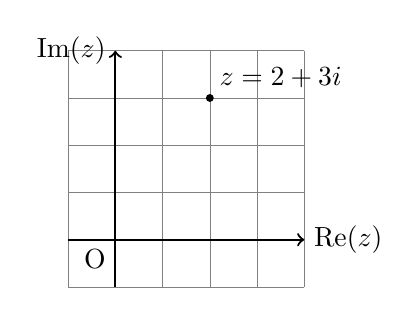
\begin{tikzpicture}[scale=.6]
        \draw[help lines] (-1, -1) grid (4, 4);
        \draw[thick, ->] (-1, 0) -- (4, 0);
        \draw[thick, ->] (0, -1) -- (0, 4);
        % \node[overlay, above] at (0, 4) {(a) Non-Zero Solution};
        \node[right] at (4, 0) {Re$(z)$};
        \node[left] at (0, 4) {Im$(z)$};        
        \node[below left] at (0, 0) {O};    
        \node[above right] at (2,3) {$z=2+3i$};    
        \filldraw (2,3) circle (.2em); 
        \end{tikzpicture}
    \end{center}    
    }
\end{frame}



\begin{frame}{Addition and Multiplication}



    \Emph{Recall}: we can add and multiply complex numbers with the usual rules.

    \medskip

    $\onslide<2->{(2-3i)+(-1+i) = } \onslide<3->{(2 - 1) + (-3 + 1)i = 1 - 2i}$

    \vspace{12pt}
    
    $\onslide<4->{(2-3i)(-1+i) =} \onslide<5->{-2+2i + }\onslide<5->{3i -3i^2 = }\onslide<6->{1 +5i} $


\end{frame}




\begin{frame}{Complex Conjugate, Absolute Value, Polar Form}

    \vspace{12pt} 

    We can \Emph{conjugate} complex numbers: $\overline{a+bi} = a - bi $ 

    \vspace{12pt} 
    
    \pause 

    The \Emph{absolute value} of a complex number: $|a+bi| = \sqrt{a^2 + b^2}$ 

    \vspace{12pt} 

    \pause 
    
    We can write complex numbers in \Emph{polar form}: $a + ib = r(\cos \phi + i\, \sin \phi)$, where: 
    
    $$r = |a+bi | \qquad \tan \phi = \frac ba$$
    
    
\end{frame}



 \begin{frame}{Complex Conjugate Properties}

     If $x$ and $y$ are complex numbers, $\vec v \in \mathbb C^n$, it can be shown that:
     \begin{itemize}
     	\item $\overline{ \left( x+ y \right) } = \overline{ x } + \overline{ y }$
     	\item $\overline{A\vec v} = A\overline{\vec v}$
    	\item Im$\left(x\overline x\right) = 0$ 
     \end{itemize}

    \vspace{12pt}
    \Emph{Example} \\ True or false: if $x$ and $y$ are complex numbers, then $$\overline{(xy)} = \overline{x} \ \overline{y}$$


 \end{frame}


\begin{frame}\frametitle{Polar Form and the Complex Conjugate}
    
    Conjugation reflects points across the real axis. 
    
    \begin{figure}[ht]
    \centering
    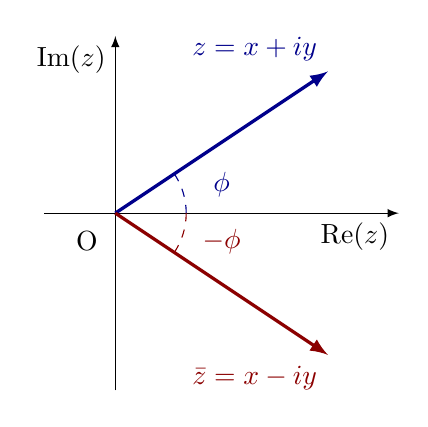
\begin{tikzpicture}[scale=0.9]
        \coordinate (Origin)   at (0,0);
        \coordinate (XAxisMin) at (-1,0);
        \coordinate (XAxisMax) at (4,0);
        \coordinate (YAxisMin) at (0,-2.5);
        \coordinate (YAxisMax) at (0,2.5);
        \draw [thin, black,-latex] (XAxisMin) -- (XAxisMax) node [below left] {Re$(z)$};% Draw x axis
        \draw [thin, black,-latex] (YAxisMin) -- (YAxisMax) node [below left] {Im$(z)$};% Draw y axis
        \coordinate (Vone) at (3,2);
        \coordinate (Vtwo) at (3,-2);        
        \draw [very thick,-latex,DarkBlue] (Origin) -- (Vone) node [above left] {$z=x+iy$};  
        \draw [very thick,-latex,DarkRed] (Origin) -- (Vtwo) node [below left] {$\bar z=x-iy$}; 
        \draw[DarkBlue,dashed] (1,0) arc (0:35:1);
        \draw[DarkRed,dashed] (1,0) arc (0:-35:1);
        \draw[DarkRed] (1.5,-0.4) node {$-\phi$};
        \draw[DarkBlue] (1.5,0.4) node {$\phi$};
        \draw[black] (-0.4,-0.4) node {O};        
    \end{tikzpicture}
    \end{figure}
\end{frame}

%  \begin{frame}\frametitle{Euler's Formula}

%     Suppose $z_1$ has angle $\phi_1$, and $z_2$ has angle $\phi_2$.  

%     \begin{figure}[ht]
%     \centering
%     \begin{tikzpicture}[scale=0.85]
%         \coordinate (Origin)   at (0,0);
%         \coordinate (XAxisMin) at (-2,0);
%         \coordinate (XAxisMax) at (4,0);
%         \coordinate (YAxisMin) at (0,-1);
%         \coordinate (YAxisMax) at (0,2.5);
%         \draw [thin, black,-latex] (XAxisMin) -- (XAxisMax) node [below left] {Re$(z)$};% Draw x axis
%         \draw [thin, black,-latex] (YAxisMin) -- (YAxisMax) node [above right] {Im$(z)$};% Draw y axis
%         \coordinate (Vone) at (2,1.3);
%         \coordinate (Vtwo) at (0.5,1.2);        
%         \coordinate (Vthr) at (-0.56,3.05);        
%         \draw [very thick,-latex,DarkBlue] (Origin) -- (Vone) node [above ] {$z_1$};  
%         \draw [very thick,-latex,red] (Origin) -- (Vtwo) node [above ] {$z_2$}; 
%         \draw [very thick,-latex,DarkGreen] (Origin) -- (Vthr) node [ left] {$z_3$}; 
%         \draw[DarkBlue] (1.2,0) arc (0:40:1);
%         \draw[red] (1.0,0) arc (0:70:1);
%         \draw[DarkGreen] (0.8,0) arc (0:90:1);
%         \draw[DarkBlue] (1.5,0.3) node {$\phi_1$};
%         \draw[red] (1,1) node {$\phi_2$};
%         \draw[black] (-0.4,-0.4) node {O};        
%     \end{tikzpicture}
%     \end{figure}
    

% The product $z_3=z_1z_2$ has angle $\phi_1 + \phi_2$ and modulus $ \lvert z\rvert \, \lvert w \rvert $. Easy to remember using Euler's formula. 
% \begin{equation*}
% \boxed{z = \lvert  z\rvert \operatorname e ^{i \phi}  }
% \end{equation*}
% The product $z_1z_2$ is:
% \begin{equation*}
% z_3 = z_1z_2 = (\lvert  z_1\rvert \operatorname e ^{i\phi_1} ) (\lvert  z_2\rvert e ^{i\phi_2} ) = \lvert z_1\rvert \, \lvert  z_2\rvert \operatorname e ^{i (\phi_1 + \phi_2)}  
% \end{equation*}
% \end{frame}






\frame{\frametitle{Summary}

    \SummaryLine \vspace{4pt}
    \begin{itemize}\setlength{\itemsep}{8pt}

    \item complex number arithmetic: addition, multiplication, complex conjugate, absolute value, polar form
    
    \item sketching complex numbers
    
    \end{itemize}
    
    \vspace{8pt}
    

    
}


